\section{Reference-branch robustness}
\label{sec:triangulation}
\label{sec:robustness}

This is the paper's centerpiece. The reconstruction above is
measured against one particular CMB-compatible history~C1. This
section repeats the comparison against a second, separately implemented
CMB-compatible history~C2 and shows the deformation is
shared. All headline metrics resolve from frozen evidence JSON through
registry macros, never handwritten.

\subsection{Endpoint invariance}

Define the logarithmic difference fields on the common grid
(Section~\ref{sec:endpoint-repr}):
\begin{equation}
  \Delta_{1}(z)=\ln H_{R}(z)-\ln H_{C1}(z),
  \label{eq:delta1}
\end{equation}
\begin{equation}
  \Delta_{2}(z)=\ln H_{R}(z)-\ln H_{C2}(z),
  \label{eq:delta2}
\end{equation}
\begin{equation}
  \Delta_{C}(z)=\ln H_{C1}(z)-\ln H_{C2}(z),
  \label{eq:deltaC}
\end{equation}
with the common and disagreement combinations
\begin{equation}
  \Delta_{\rm common}(z) = \frac{\Delta_{1}(z)+\Delta_{2}(z)}{2},
  \label{eq:common}
\end{equation}
\begin{equation}
  \Delta_{\rm disagreement}(z) = \frac{\Delta_{1}(z)-\Delta_{2}(z)}{2}.
  \label{eq:disagreement}
\end{equation}
The quoted common-mode fraction is
\begin{equation}
  f_{\rm common}
  =
  1-
  \left[
  \frac{\mathrm{RMS}(\Delta_{\rm disagreement})}
       {\mathrm{RMS}(\Delta_{\rm common})}
  \right]^2,
  \label{eq:fcommon}
\end{equation}
evaluated per redshift interval on the constrained domain.
Changing the CMB reference branch from C1 to C2 does not change the
hypothesis: the same compact map must describe both separations.

\subsection{Common-mode decomposition}

On the constrained domain ($z\le1.8$), the two R--CMB fields lie
substantially on top of one another. The common-mode fraction
exceeds~\GeometryCommonFractionMin{} in every redshift interval, and
the two-vector singular decomposition is dominated by a single
shared direction (dominance ratio~\GeometrySvdDominance{}). The two
fields peak at the same location, near
$z\approx\GeometryPeakZ{}$, while across the constrained bins the
CMB--CMB RMS difference is about 1--8\% of the R--CMB difference (RMS ratios
\GeometryCmbRatioLow{} on the peak interval and
\GeometryCmbRatioHigh{} at high redshift).

\subsection{Peak location and data support}
\label{sec:peak-support}

The fitted difference reaches its largest amplitude near
$z\approx\GeometryPeakZ{}$. Because this region also carries
substantial observational leverage, we do not interpret the peak
redshift as a fundamental physical scale. A bounded diagnostic
(peak-support summary in paper evidence,
no refitting) compares the frozen peak against Pantheon+ SN count
and inverse-variance densities, DESI BAO information density and
block locations, and the already-computed fit-improvement attribution: the peak
does not coincide with any simple data-density maximum. The
recorded disposition is peak-not-explained-by-simple-data-density.
R--C1 and R--C2 both peak near $0.65$; the frozen m3 curve (maximum
near $0.39$) captures their broad low/intermediate-$z$ trend but not
their exact peak. The peak's origin remains unresolved.

\subsection{Cross-branch transfer}

The frozen order-3 basis transfers across branches: shape amplitudes
refit independently agree, and parameters learned on one CMB branch
predict the other separation with residual degradation fraction
\GeometryTransferDegradation{} ($\le 6.8\%$ cross-branch). One
dominant shared direction carries the deformation; the residual
branch-specific component is small.

\subsection{Statistical status of the reference-branch robustness test}
\label{sec:robustness-stats}

The m3 order-selection bootstrap tests model complexity; it does not
test reference-construction similarity. The reference-sensitivity metrics quantify robustness of frozen
best-fit histories: how much the measured R--CMB separation moves
when the CMB reference construction changes. C1 and C2 are not
statistically independent (both use Planck information;
Section~\ref{sec:endpoint-c2}), and the two difference fields share
the same R endpoint ($\Delta_{1}=R-C_{1}$,
$\Delta_{2}=R-C_{2}$), so their similarity is mathematically
correlated. Endpoint posterior uncertainty was not propagated.
Therefore no frequentist p-value is assigned to the cosine or
common-mode statistic. The reference-branch robustness test shows a
shared low-dimensional deformation across the tested constructions;
it does not confirm a theory.

\subsection{Constrained domain and Ly$\alpha$ continuation}

All reference-sensitivity metrics above are quoted on the constrained
domain $z\le1.8$, covering every non-Ly$\alpha$ DESI block. The
Ly$\alpha$ anchor at $z=2.33$ is a continuation test of the
reconstruction law, not a measurement of the low-redshift
deformation: flexible extrapolators generically fail there, under
the null as on the data (Ly$\alpha$ catastrophe fraction
\CvConstrLyaProb{} in the matched constrained-domain bootstrap,
recorded separately and never used in selection).

\subsection{Comparison with the fit-improvement attribution}

The deformation RMS (peak bin $0.4<z<0.8$) and the
fit-improvement attribution (peak bin $0<z<0.4$) both concentrate
below $z\sim0.8$, though their peak bins differ; high-redshift behavior
is unconstrained in both. The reference-sensitivity check therefore supports, rather
than replaces, the compact reconstruction: the same
five-coordinate map describes a deformation that is
reference-insensitive within the two tested Planck-compatible constructions.

\begin{figure}[!htbp]
  \centering
  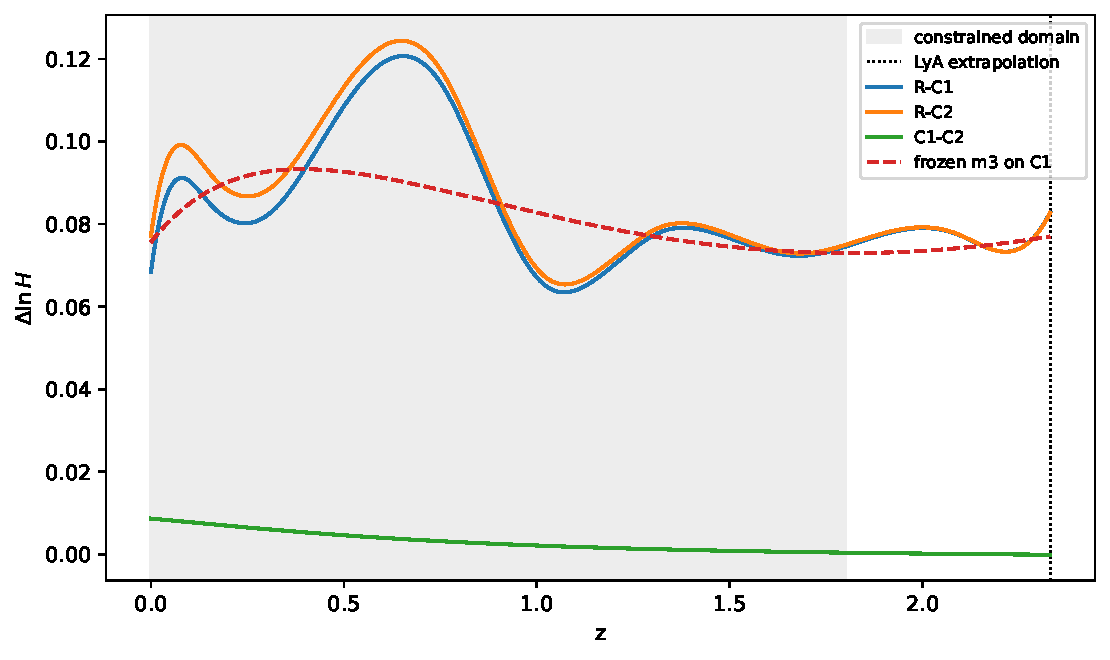
\includegraphics[width=0.9\linewidth]{figures/generated/bridge_fig5_triangulation}
  \caption{Reference-sensitivity overlay: the two R--CMB difference fields
  lie on top of one another across the constrained domain (R--C1 and
  R--C2 nearly coincide; C1--C2 is much smaller), and the
  frozen m3 reconstruction captures the broad low/intermediate-redshift
  trend but not the exact peak near $z\simeq0.65$. Shading marks the
  constrained domain; the dotted line marks the Ly$\alpha$
  extrapolation test.}
  \label{fig:bridge-triangulation}
\end{figure}
